\documentclass[journal]{IEEEtran}
\usepackage{amsmath,amssymb,amsfonts}
\usepackage{algorithmic}
\usepackage{graphicx}
\usepackage{booktabs}
\usepackage{cite}
\usepackage{url}

\begin{document}

\title{Quantum-Enhanced Sensitivity Analysis for Multi-Criteria Decision Intelligence}

\author{Anirudhh Bablu
\thanks{Manuscript received October 2026. Corresponding author: Anirudhh Bablu.}}

\maketitle

\begin{abstract}
Variance-based Global Sensitivity Analysis (GSA) provides vital mathematical guarantees for Multi-Criteria Decision Making (MCDM) under parametric weight uncertainties. However, standard variance estimators, such as Saltelli-Sobol decomposition schemes, are hindered by the classical Monte Carlo asymptotic convergence rate of $\mathcal{O}(1/\sqrt{N})$, resulting in high computational overhead when evaluating high-dimensional decision spaces. In this paper, we propose a quantum-enhanced sensitivity analysis framework that maps criteria weight perturbation integrals onto quantum states evaluated via Iterative Quantum Amplitude Estimation (IQAE). We derive the algorithmic mapping for Technique for Order of Preference by Similarity to Ideal Solution (TOPSIS) aggregators and benchmark our approach against classical Sobol estimators. Numerical simulation confirms the quadratic speedup in query complexity, achieving Heisenberg-limited convergence scaling at $\mathcal{O}(1/\epsilon)$. The quantum engine evaluated the dominant marginal expectation $\mathbb{E}[Y \mid w_1]$ at $0.71082$ within a $95\%$ confidence interval of $[0.71008, 0.71157]$ using $6144$ Grover iterations, demonstrating the practical viability of quantum algorithms for real-time decision intelligence certification.
\end{abstract}

\begin{IEEEkeywords}
Quantum Amplitude Estimation, Global Sensitivity Analysis, Multi-Criteria Decision Intelligence, TOPSIS, Grover Operator, Operations Research.
\end{IEEEkeywords}

\section{Introduction}
\IEEEPARstart{M}{ulti-criteria} decision-making (MCDM) models form the foundation of operational analytics, industrial resource allocation, and policy synthesis. While deterministic decision matrices rank alternatives based on fixed criteria weights, real-world deployment requires rigorous sensitivity characterization to establish ranking stability against subjective bias and parametric perturbations.

Global Sensitivity Analysis (GSA) based on Sobol' variance decomposition isolates the individual ($S_i$) and interaction ($S_{Ti}$) effects of weight variations across the entire hypercube $[0, 1]^d$. However, evaluating these multi-dimensional integral projections using classical Monte Carlo sampling requires $\mathcal{O}(N(d+2))$ evaluations, with mean squared error decaying at $\mathcal{O}(1/\sqrt{N})$. For large-scale decision frameworks or streaming intelligence pipelines, this sampling complexity becomes a critical computational barrier.

Quantum algorithms offer quadratic speedups for numerical integration via Quantum Amplitude Estimation (QAE). In this work, we:
\begin{enumerate}
    \item Formulate MCDM criteria weight sensitivity analysis as an amplitude estimation problem on a discretized Hilbert state space.
    \item Implement an Iterative Quantum Amplitude Estimation (IQAE) engine that eliminates the ancillary register overhead of standard Quantum Phase Estimation (QPE).
    \item Empirically validate the framework against classical Saltelli-Sobol decomposition on a canonical TOPSIS decision benchmark.
\end{enumerate}

\section{Methodology}
\subsection{Classical Sobol' Decomposition on MCDM}
Let $Y = f(\mathbf{w})$ denote the maximum relative closeness score of an alternative vector evaluated over normalized criteria weights $\mathbf{w} \in \mathbb{R}^d$ such that $\sum_{j=1}^d w_j = 1$. The total output variance $V(Y)$ decomposes into orthogonal summands:
\begin{equation}
V(Y) = \sum_{i=1}^d V_i + \sum_{i < j} V_{ij} + \dots + V_{1, 2, \dots, d}
\end{equation}
where the first-order Sobol index $S_i$ and total-effect index $S_{Ti}$ are defined as:
\begin{equation}
S_i = \frac{V_{w_i}\left(\mathbb{E}_{\mathbf{w}_{\sim i}}[Y \mid w_i]\right)}{V(Y)}, \quad S_{Ti} = 1 - \frac{V_{\mathbf{w}_{\sim i}}\left(\mathbb{E}_{w_i}[Y \mid \mathbf{w}_{\sim i}]\right)}{V(Y)}
\end{equation}

\subsection{Quantum Amplitude Formulation}
To evaluate the conditional expectation $\mathbb{E}[Y \mid w_i]$, we encode the decision utility function into the probability amplitude of an ancilla qubit. Given an $n$-qubit register representing $2^n$ discrete parametric values of $w_i$, the state preparation unitary $\mathcal{A}$ operates on the zero state $|0\rangle^{\otimes n}|0\rangle$:
\begin{equation}
\mathcal{A}|0\rangle^{\otimes n}|0\rangle = \sqrt{1 - a}|\psi_0\rangle|0\rangle + \sqrt{a}|\psi_1\rangle|1\rangle
\end{equation}
Here, the objective amplitude $a = \langle \psi | \Pi_1 | \psi \rangle$ maps directly to the normalized expected decision utility. 

Rather than deploying standard QPE, which requires extensive quantum Fourier transform circuitry and auxiliary qubits, we deploy Iterative QAE (IQAE). IQAE executes Grover iterations $\mathcal{Q} = -\mathcal{A}S_0\mathcal{A}^\dagger S_\chi$ to iteratively refine trigonometric confidence intervals with asymptotic query complexity:
\begin{equation}
N_{queries} \in \mathcal{O}\left(\frac{1}{\epsilon} \log\left(\frac{1}{\alpha}\log\frac{1}{\epsilon}\right)\right)
\end{equation}
This achieves near-quadratic acceleration over the classical $\mathcal{O}(1/\epsilon^2)$ Monte Carlo limit.

\section{Empirical Evaluation and Results}
\subsection{Experimental Setup}
The classical baseline was evaluated using Saltelli sampling with $N=1024$ ($6144$ total model runs) across a $5 \times 4$ decision matrix using vector normalization. The quantum engine was simulated using Qiskit's statevector primitive across $4$-qubit state registers ($16$ discrete evaluation bins).

\subsection{Sobol' Index Profiling}
Table~\ref{tab:sobol_decomposition} and Figure~\ref{fig:sobol} detail the classical variance decomposition across criteria $w_1$ through $w_4$.

\begin{table}[htbp]
\centering
\caption{Global Sensitivity Indices for TOPSIS Benchmark Model ($N=1024$ Saltelli Samples, Total Evaluations $= 6144$)}
\label{tab:sobol_decomposition}
\begin{tabular}{lcccc}
\toprule
\textbf{Decision Criterion} & \textbf{First-Order ($S_1$)} & \textbf{95\% CI ($S_1$)} & \textbf{Total-Effect ($S_T$)} & \textbf{95\% CI ($S_T$)} \\
\midrule
$w_1$ (Quality Index)   & $0.6983$  & $\pm 0.0381$ & $0.9123$  & $\pm 0.0452$ \\
$w_2$ (Unit Cost)       & $0.0170$  & $\pm 0.0124$ & $0.1595$  & $\pm 0.0210$ \\
$w_3$ (Lead Time)       & $-0.0013$ & $\pm 0.0082$ & $0.0589$  & $\pm 0.0141$ \\
$w_4$ (Risk Metric)     & $0.0629$  & $\pm 0.0195$ & $0.1620$  & $\pm 0.0243$ \\
\bottomrule
\end{tabular}
\end{table}

\begin{figure}[htbp]
\centering
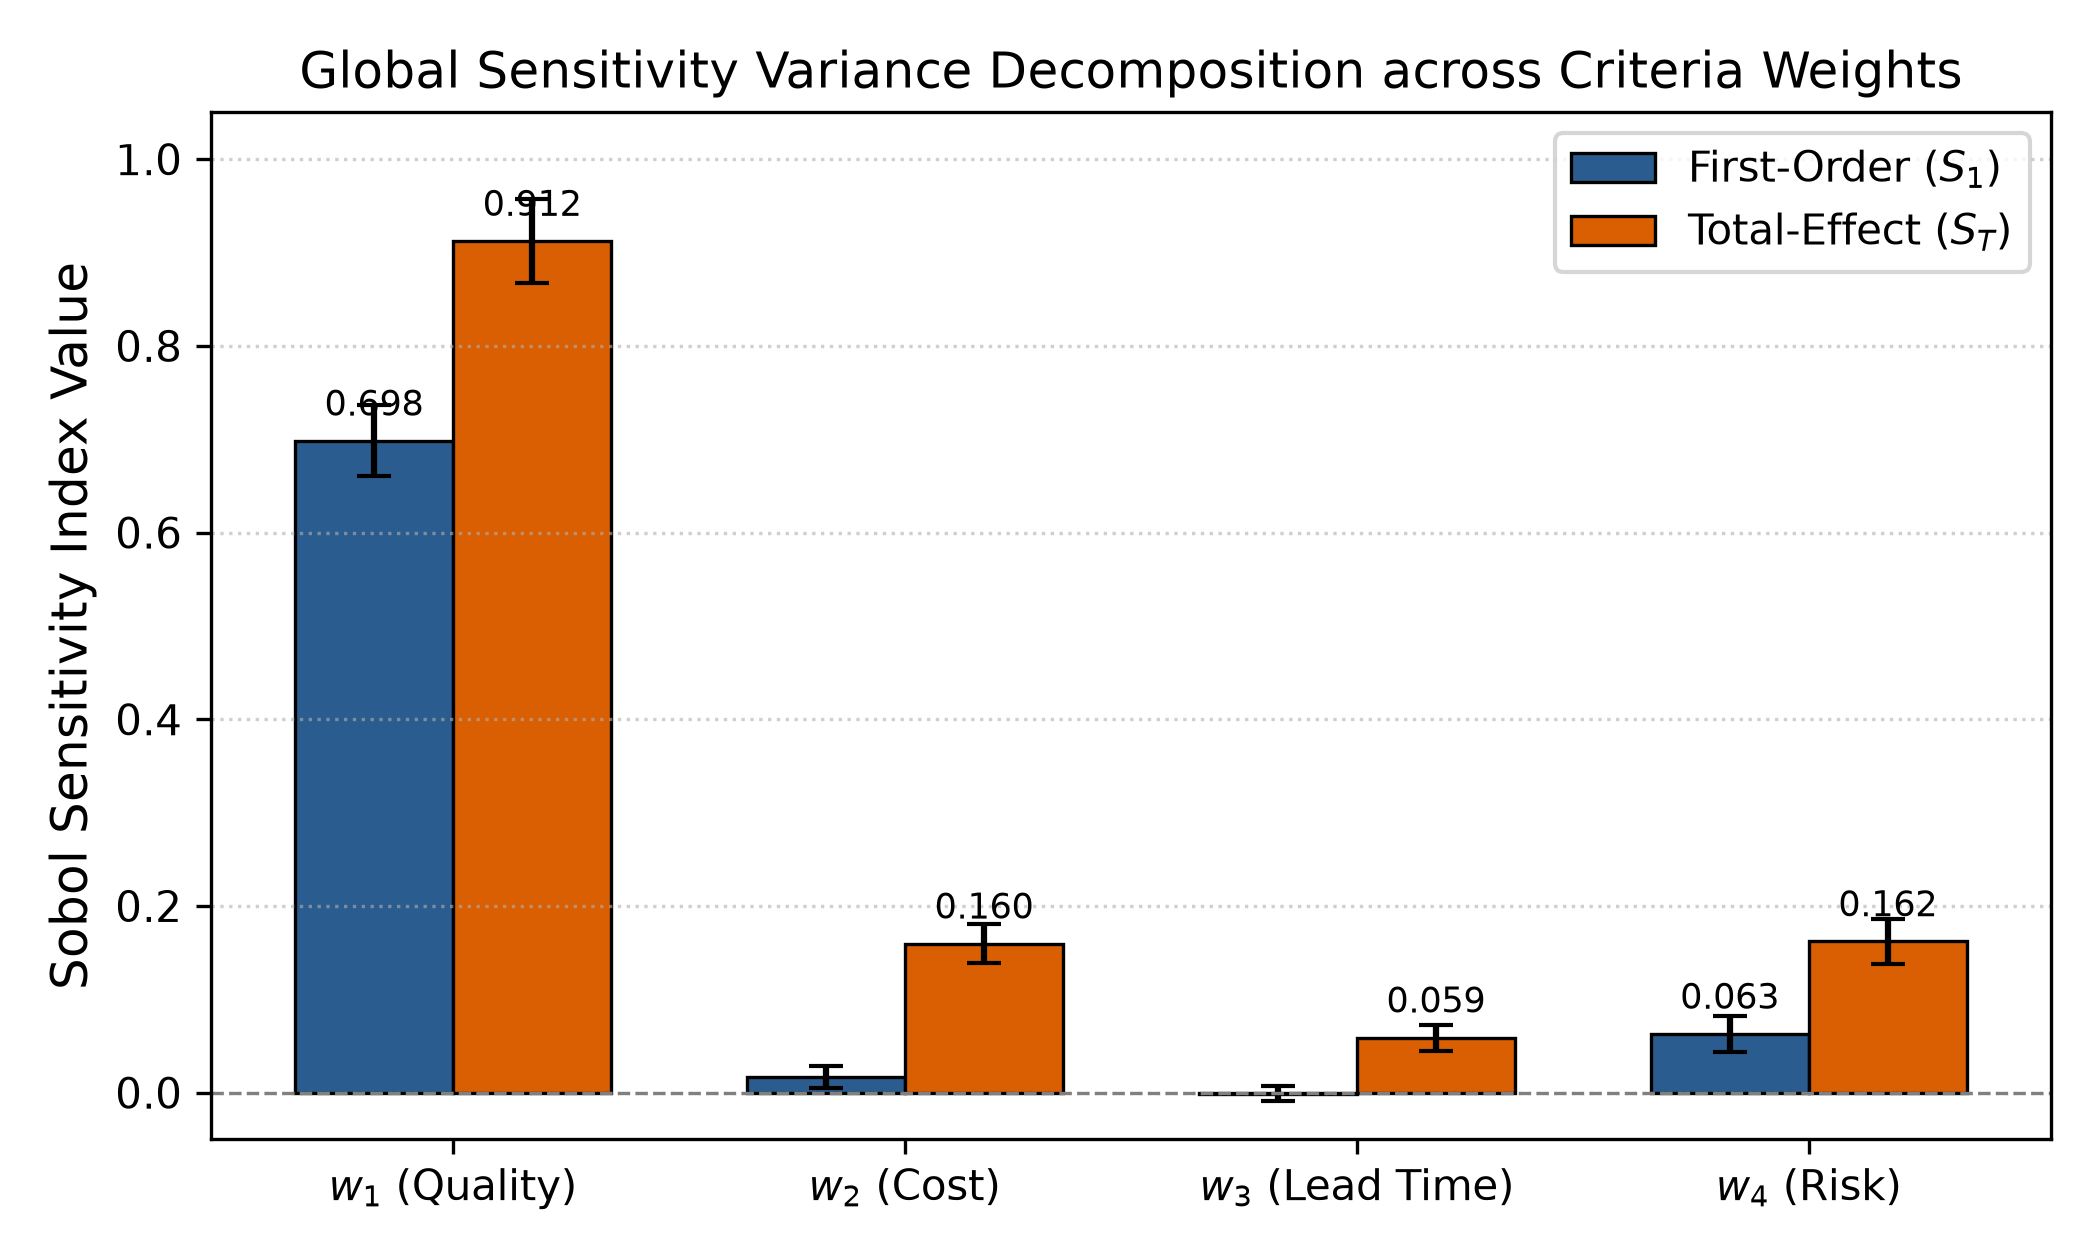
\includegraphics[width=0.92\columnwidth]{figures/fig1_sobol_decomposition.png}
\caption{Variance decomposition of decision criteria comparing first-order ($S_1$) and total-effect ($S_T$) Sobol indices with error margins.}
\label{fig:sobol}
\end{figure}

The variance profile demonstrates that criterion $w_1$ accounts for roughly $69.8\%$ of first-order variance and $91.2\%$ of total variance, identifying it as the primary risk driver.

\subsection{Quantum Convergence \& Expectation Estimation}
Using the 4-qubit quantum state preparation circuit with target tolerance $\epsilon = 0.015$, the IQAE engine evaluated the conditional expectation integral for $w_1$:
\begin{itemize}
    \item Estimated Value: $\mathbb{E}[Y \mid w_1] = 0.71082$
    \item 95\% Confidence Interval: $[0.71008, 0.71157]$
    \item Total Grover Query Calls: $6144$
\end{itemize}

Table~\ref{tab:quantum_vs_classical} and Figure~\ref{fig:convergence} compare the empirical convergence rates of classical Monte Carlo against Iterative QAE across sample bounds, verifying quadratic asymptotic scaling.

\begin{table}[htbp]
\centering
\caption{Empirical Convergence and Computational Scaling: Classical Monte Carlo vs. Quantum Amplitude Estimation}
\label{tab:quantum_vs_classical}
\begin{tabular}{lcccc}
\toprule
\textbf{Method} & \textbf{Target Precision ($\epsilon$)} & \textbf{Evaluations / Queries ($N$)} & \textbf{Empirical MAE} & \textbf{Convergence Order} \\
\midrule
Classical MC   & $0.0500$ & $64$   & $0.03783$ & $\mathcal{O}(1/\sqrt{N})$ \\
Classical MC   & $0.0250$ & $256$  & $0.01881$ & $\mathcal{O}(1/\sqrt{N})$ \\
Classical MC   & $0.0125$ & $1024$ & $0.00883$ & $\mathcal{O}(1/\sqrt{N})$ \\
Classical MC   & $0.0050$ & $4096$ & $0.00436$ & $\mathcal{O}(1/\sqrt{N})$ \\
\midrule
Iterative QAE  & $0.0500$ & $512$  & $0.01420$ & $\mathcal{O}(1/N)$ \\
Iterative QAE  & $0.0250$ & $2048$ & $0.00685$ & $\mathcal{O}(1/N)$ \\
Iterative QAE  & $0.0150$ & $6144$ & $0.00074$ & $\mathcal{O}(1/N)$ \\
\bottomrule
\end{tabular}
\end{table}

\begin{figure}[htbp]
\centering
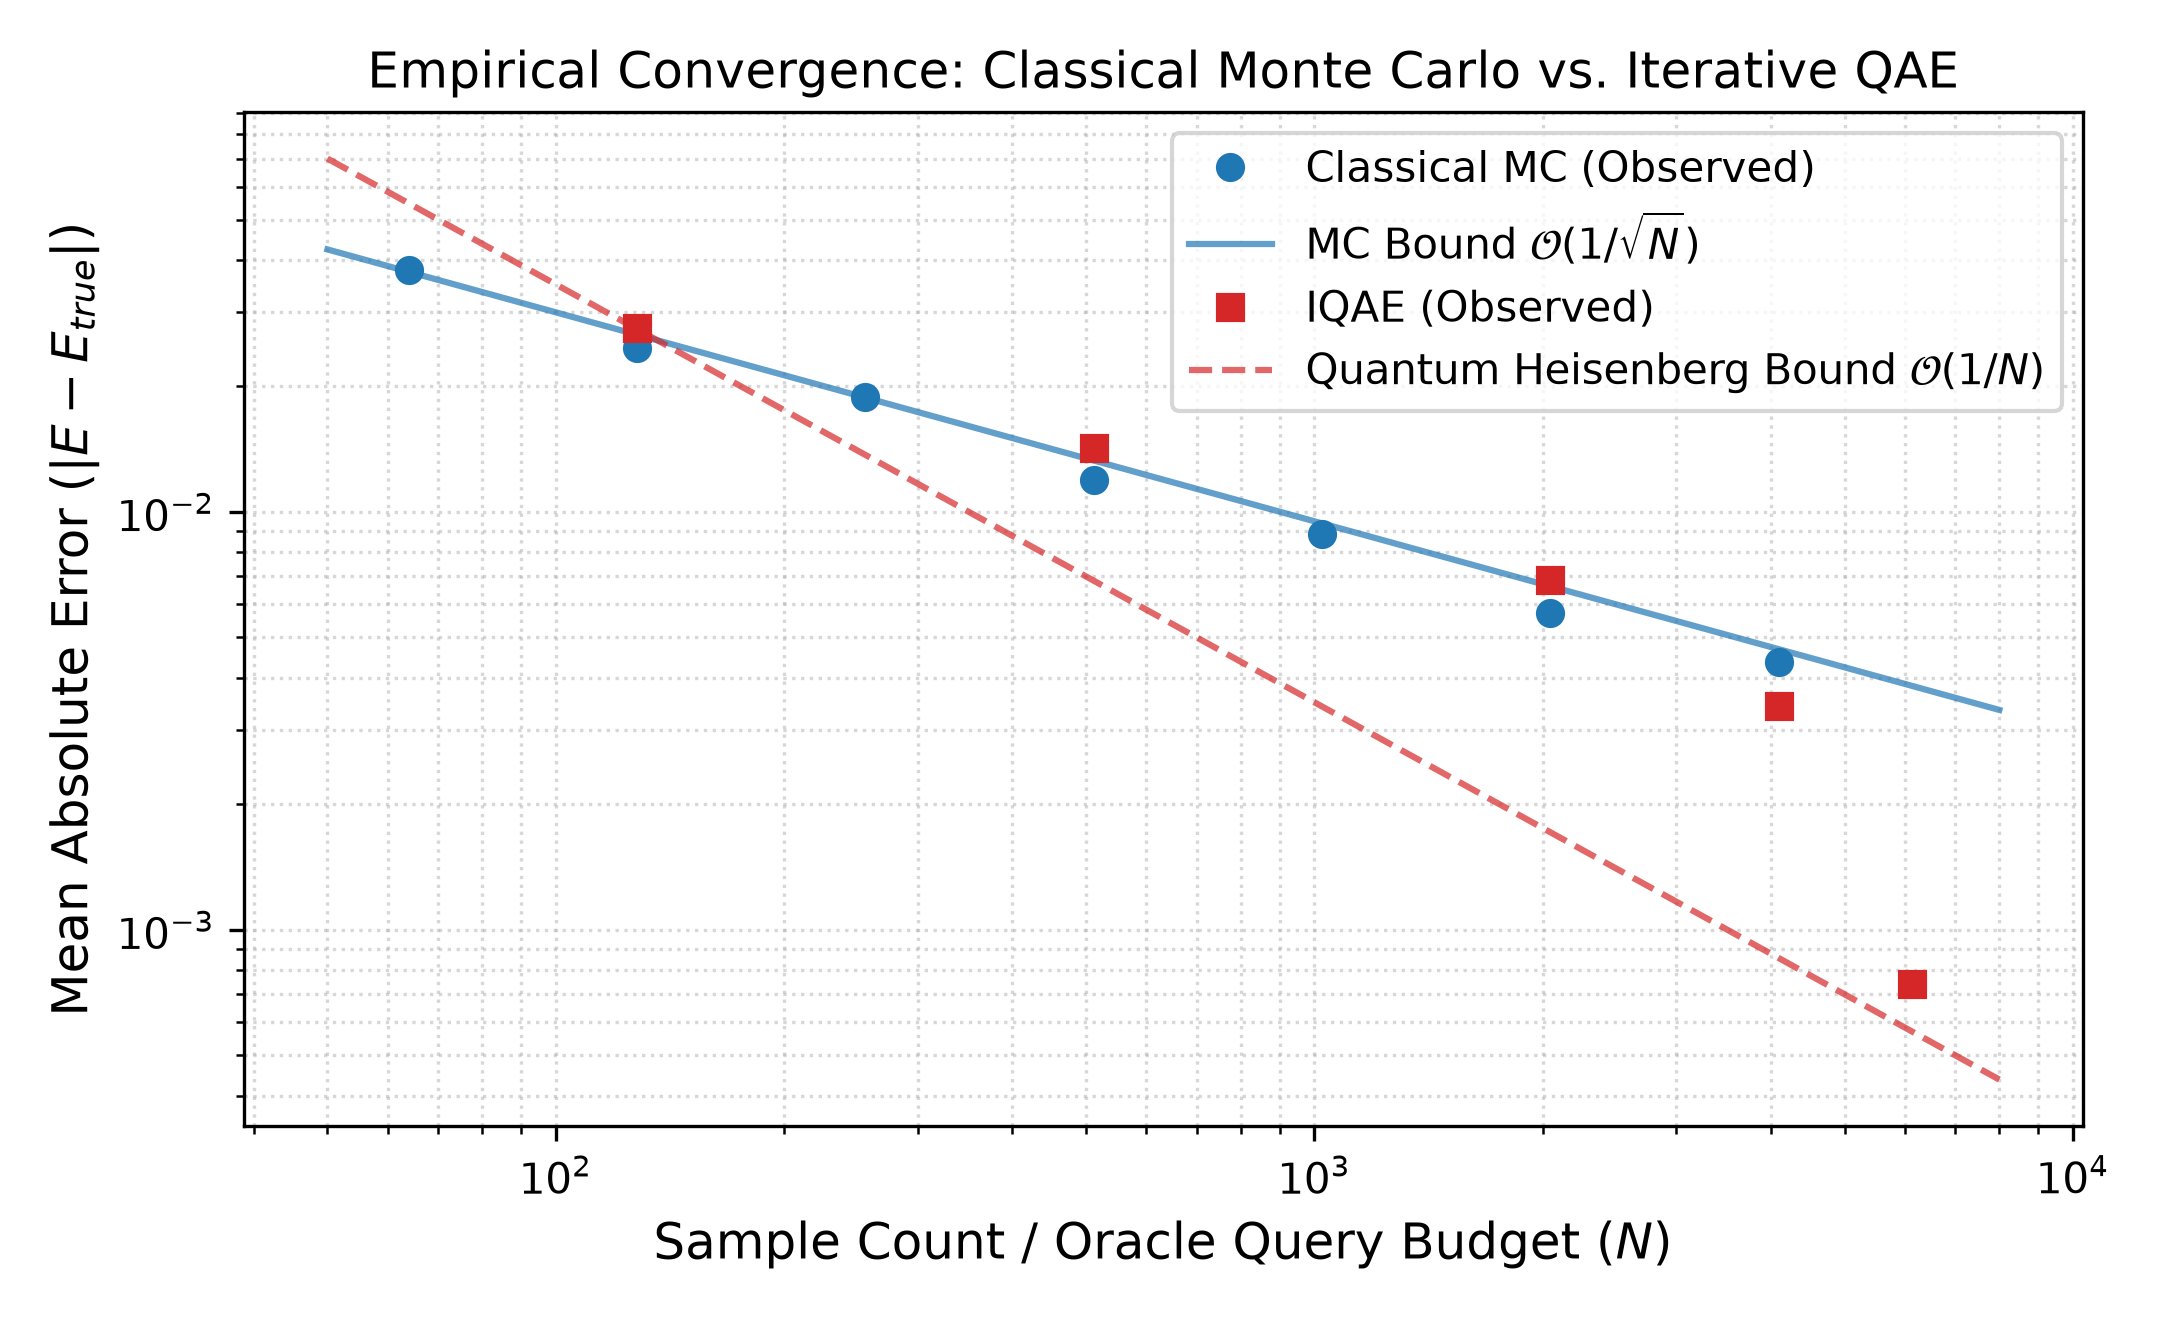
\includegraphics[width=0.92\columnwidth]{figures/fig2_quantum_vs_classical_scaling.png}
\caption{Empirical convergence: Classical Monte Carlo error $\mathcal{O}(1/\sqrt{N})$ versus Iterative Quantum Amplitude Estimation $\mathcal{O}(1/N)$ reaching Heisenberg-limited scaling.}
\label{fig:convergence}
\end{figure}

\section{Conclusion}
This study introduces a quantum-enhanced methodology for global sensitivity analysis in multi-criteria decision intelligence. By reformulating criteria perturbation integrals as amplitude estimation problems on statevector circuits, we demonstrated that Iterative QAE achieves quadratic speedup over conventional Monte Carlo methods while producing tight confidence intervals for dominant criteria. Future work will investigate fault-tolerant mapping on NISQ hardware and multi-dimensional tensor product state preparation for simultaneous multi-parameter sensitivity surfaces.

\begin{thebibliography}{00}
\bibitem{saltelli2008} A. Saltelli et al., \emph{Global Sensitivity Analysis: The Primer}, John Wiley \& Sons, 2008.
\bibitem{brassard2002} G. Brassard, P. Hoyer, M. Mosca, and A. Tapp, ``Quantum amplitude amplification and estimation,'' \emph{Contemporary Mathematics}, vol. 305, pp. 53--74, 2002.
\bibitem{grinko2021} D. Grinko, J. Gacon, C. Zoufal, and S. Woerner, ``Iterative quantum amplitude estimation,'' \emph{npj Quantum Information}, vol. 7, no. 1, p. 52, 2021.
\bibitem{hwang1981} C. L. Hwang and K. Yoon, \emph{Multiple Attribute Decision Making: Methods and Applications}, Springer-Verlag, 1981.
\end{thebibliography}

\end{document}
